\chapter{总线}\label{CO06}

\par\medskip\noindent\textbf{知识导图}\par\smallskip
\begin{wideblock}\centering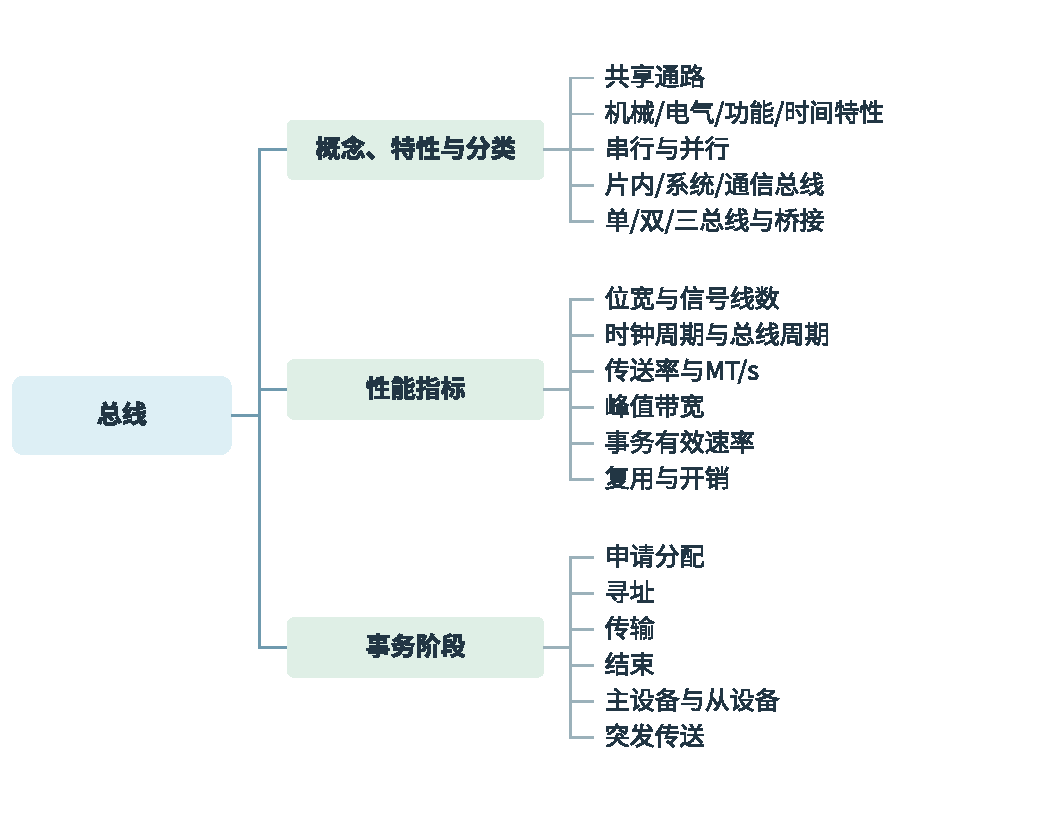
\includegraphics[width=\linewidth,height=168mm,keepaspectratio]{figures/map-01.pdf}\end{wideblock}\par\medskip\clearpage

\par\medskip\noindent\textbf{知识导图（续）}\par\smallskip
\begin{wideblock}\centering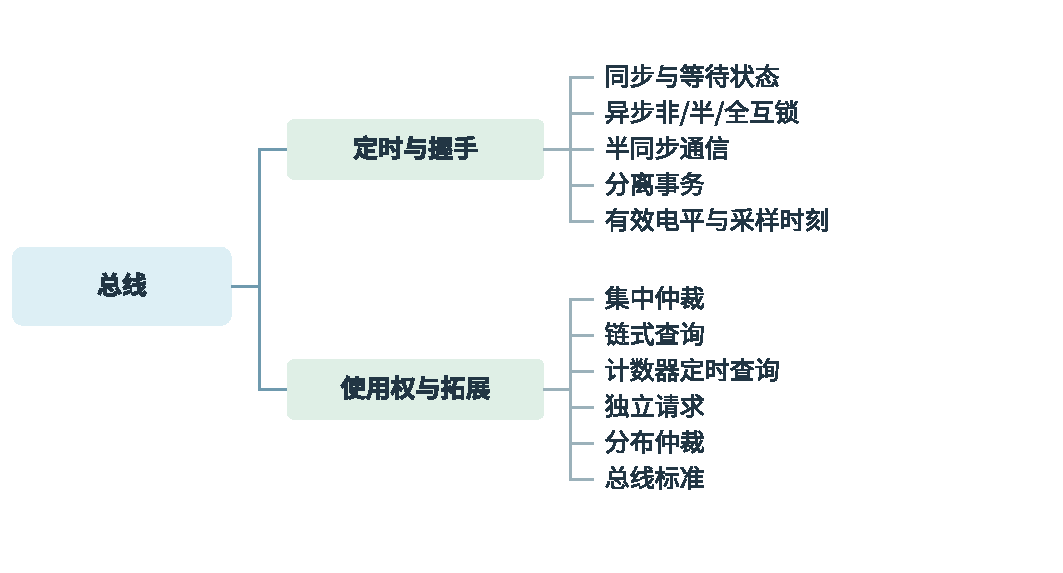
\includegraphics[width=\linewidth,height=168mm,keepaspectratio]{figures/map-02.pdf}\end{wideblock}\par\medskip\clearpage

\section{从概念、性能到事务时序}\label{CO06-map}

本章沿课件导图的四组关系展开：先由``共享通路''辨认总线的组成、分类与结构，再把位宽、周期和传送率写成可计算的量，随后按申请、寻址、传输、结束四阶段追踪一次事务。定时方式回答``何时允许推进''；仲裁回答``由谁取得使用权''，两者分属不同问题。

\begin{definition}[总线的共享性]

总线是一组能被多个部件分时共享的信息传送通路。连接在同一条公共通路上，不表示多个主设备可以同时任意驱动线路；同一时刻允许的驱动者、接收者及信号解释由协议决定。

\end{definition}

总线特性可以按四个维度检查：机械特性规定连接器、尺寸和形状；电气特性规定电平、负载等；功能特性规定每根线承载什么；时间特性规定信号建立、采样及撤销关系。它们分别回答``如何接、什么电平、传什么、何时有效''。

按位置与用途可分片内总线、连接CPU/主存/I/O接口的系统总线，以及部件或系统间的通信通路；按数据形式分串行与并行；按定时分同步、异步等。一个具体接口可以同时具有``串行''``包传输''``多通道''的属性，分类维度不能混为一个互斥列表。

单总线结构让多个部件共享一条系统通路，连接简单但易形成争用；双总线、三总线以不同层次分担主存和I/O等流量。桥接器完成不同总线间的数据缓冲、协议转换和控制。增加通路能减少某类冲突，仍须核对桥接和主存是否成为瓶颈。

\section{位宽、频率、传送率分别给出什么}\label{CO06-metrics}

总线是部件之间传送信息的公共通路。按信息用途可区分地址、数据和控制：地址说明访问哪个单元或端口，数据线承载被交换的值，控制线说明操作类型、有效时刻及应答等。命令字虽然在语义上``控制设备''，CPU写命令字时仍可能在\textbf{数据线}上传送；不能只凭名称判断该走哪组线。

数据线上可以传指令、操作数、状态字、命令字和中断类型号。它们如何解释取决于传送双方和操作类型。MAR保存待访问地址，MDR暂存交换的值；主存并不靠``某个数据看起来像地址''来判定这次访问的性质，而是由相应线路与控制时序确定。

总线位宽通常指并行数据线根数。串行传送逐位使用通道，并行传送同一时刻通过多条线传若干位；多个串行通道并用，并不等于一条传统并行总线。系统可用桥接部件连接不同速度和协议的通路，靠近CPU的部件通常要求更高带宽；有多条总线，并不表示它们共用同一时钟。

{\tcbset{SNbase/.append style={breakable=false}}\begin{methodbox}[带宽先写每次字节数与每秒次数]

若有效数据宽度为 W 位，每秒实际发生 R 次数据传送，理想单方向峰值带宽为 \(R\times W/8\) B/s。R 与时钟频率不一定相同：每周期一次为R=f，每周期两次为R=2f；若已给MT/s，则已经是每秒传送次数，不能再乘``每周期次数''。

总线周期是一次规定的总线操作所占的时间，可能有多个时钟周期。带宽为每次传送的有效数据量除以这次所用时间；控制、地址、等待、校验与空闲开销会使有效数据率低于只算数据节拍的峰值。

\end{methodbox}}

\subsection{例 6-1　一个总线周期占两个时钟周期}\label{CO06-example-1}

【配套例题】 假设某系统总线在一个总线周期中并行传输4 B信息，一个总线周期占用2个时钟周期，总线时钟频率为10 MHz，则总线带宽是（　）。

A. 10 MB/s　 B. 20 MB/s　 C. 40 MB/s　 D. 80 MB/s

\textbf{解析。} 时钟周期100 ns，一次总线传送需200 ns，传4 B，因此带宽 \(4/(200\times10^{-9})=20\times10^6\) B/s，选 \textbf{B}。若直接用4 B\ensuremath{\times}10 MHz，就忽略了每次传送占两拍。

\subsection{例 6-2　已给传送率时不重复乘每周期次数}\label{CO06-example-2}

\begin{example}[自拟数值例]

某64位并行总线每时钟周期传4次数据，实际数据传送率已明确给为1333 MT/s，求单方向理想峰值带宽。若改给的是333.25 MHz时钟频率，结果是否相同？

\end{example}

\textbf{解析。} 每次64位=8 B；1333 MT/s就是每秒 \(1333\times10^6\) 次，带宽为 \(1333\times10^6\times8=10.664\) GB/s。若给333.25 MHz且每拍4次，则先算 \(R=4f=1333\) MT/s，结果相同。若改成1333 MHz时钟、仍每拍4次，才会得到42.656 GB/s。三个单位条件必须分别使用，不能把``频率''字样覆盖题干明示的物理量。

多通道带宽只有在各通道能够并行传送且工作分配允许时才相加。全双工总线要区分单方向带宽和两个方向合计带宽；校验位若不属于有效载荷，不应计入有效数据量的分子。带宽题第一步宜写出``每次有效几字节、每秒几次''，再统一单位。

\section{一次总线事务从地址到应答}\label{CO06-transaction}

总线主设备发起事务，从设备按地址被选中并完成操作。CPU常是主设备，DMA控制器也可在取得使用权后成为主设备。主从关系只就本次事务而言，不等于某个设备永久只能发送或只能接收。

一次读事务可以分为：主设备发地址和读命令；从设备译码并准备数据；从设备在数据线上给出有效数据；主设备采样，双方结束本轮操作。写事务则由主设备给出要写的数据。地址、数据若复用同一组线路，就需不同时间片分别传送，不能把这些线路同时算成两份独立的并行位宽。

\subsection{同步定时：固定采样时刻，必要时插等待}\label{CO06-sync}

同步总线用共同的时钟约定信号的有效和采样时刻。最短周期必须覆盖信号传播、译码、设备准备及建立时间等延迟。若从设备来不及，可按协议插入等待状态；``同步''不等于所有事务长度永远相同，也不表示每个设备可随意提供互不协调的时钟。

突发传送只给出一个首地址，再连续传送多个相邻数据，分摊地址和启动开销。非突发则可能为每个数据重复地址及准备过程。因此``读一块多长时间''应先数数据拍数，再判断地址、等待代价要付几遍。

\subsection{例 6-3　不支持突发，就要反复准备每个数据}\label{CO06-example-3}

【配套例题】 某存储器总线宽度为64位，总线时钟频率为1 GHz，在总线上传输一个数据或地址需要一个时钟周期，不支持突发传送方式。若通过该总线连接CPU和主存，主存每次准备一个64位数据需要6 ns，主存块大小为32 B，则读取一个主存块所需的时间是（　）。

A. 8 ns　 B. 11 ns　 C. 26 ns　 D. 32 ns

\textbf{解析。} 一拍1 ns，每个64位数据为8 B，一块需要4个数据。每个数据都单独付地址1 ns、准备6 ns、传送1 ns，共8 ns，总计 \(4\times8=32\) ns，选 \textbf{D}。11 ns对应只付一次地址和准备、再连传4次，是突发模型，题目已排除。

\subsection{例 6-4　峰值带宽与整次事务的有效速率}\label{CO06-example-4}

【配套例题】 某存储器总线的时钟频率为420 MHz，总线宽度为64位，每个时钟周期传送2次数据；其总线事务支持突发传送方式，最多传送8次数据，第1个时钟周期传送地址和读/写命令，从第4个至第7个时钟周期连续传送8次数据。该总线的总线带宽（最大数据传输率）为（　）。

A. 3.84 GB/s　 B. 6.72 GB/s　 C. 30.72 GB/s　 D. 53.76 GB/s

\textbf{解析。} 问的是数据节拍的最大传送率，每周期2次、每次8 B，峰值 \(420\times10^6\times2\times8=6.72\) GB/s，选 \textbf{B}。

若另问这次8次数据的事务有效速率，才把地址和等待计入分母：数据64 B、事务7周期，\(64/(7/(420\times10^6))=3.84\) GB/s。A正是按整次事务口径算出的结果，不能用它回答本题已经说明的峰值带宽。第4至第7拍共4拍，每拍2次，正好8次，不是8拍。

\subsection{峰值、事务速率与CPU占用采用不同分母}\label{ux5cf0ux503cux4e8bux52a1ux901fux7387ux4e0ecpuux5360ux7528ux91c7ux7528ux4e0dux540cux5206ux6bcd}

总线峰值带宽按数据节拍可持续搬多少有效字节来计，事务有效速率还把本次地址、等待等时间算入；设备速率是设备产生或消耗数据的速度；CPU占用率则是CPU执行查询、服务或设置收尾的时间比例。这四个量可能出现在同一道题中，应先分别写成``什么量除以什么时间''。

例如在例 6-4中数据节拍峰值6.72 GB/s、整次事务有效速率3.84 GB/s，都不能直接当成某个设备的实测速率；若设备只提供40 MB/s，系统还受这个供数速度限制。反过来，DMA可让设备数据直接经过总线进入主存，同时CPU仅做少量设置收尾，所以不能把总线使用率等同于CPU使用率。端到端吞吐要核最慢环节，资源占用要核实际争用的时段。

当一次突发在等待期间必须保持总线占有权时，等待也消耗总线资源；若题设明确采用分离事务、允许准备期间让出总线，则总历时与实际占用时间还会不同。画事务时间线时，应同时标出``在等什么''和``谁仍占有总线''，不能仅凭延迟长短直接推断总线忙碌比例。

\subsection{异步定时：用握手确认进度}\label{CO06-async}

异步总线不用统一周期来强制双方同拍完成，而用请求和应答等信号交换进度。速度较慢的设备晚些应答，主设备相应等待。异步仍受顺序约束，也不能随时改变信号而不通知对方。

全互锁的四阶段握手可以写为：主设备置请求；从设备准备好后置应答；主设备看到应答后撤请求；从设备看到请求撤销后撤应答。各阶段都等待对方作出相应反应，因而不依赖预设的固定延迟来猜测对方已结束。

\par\medskip\noindent\begin{minipage}{\linewidth}
\centering
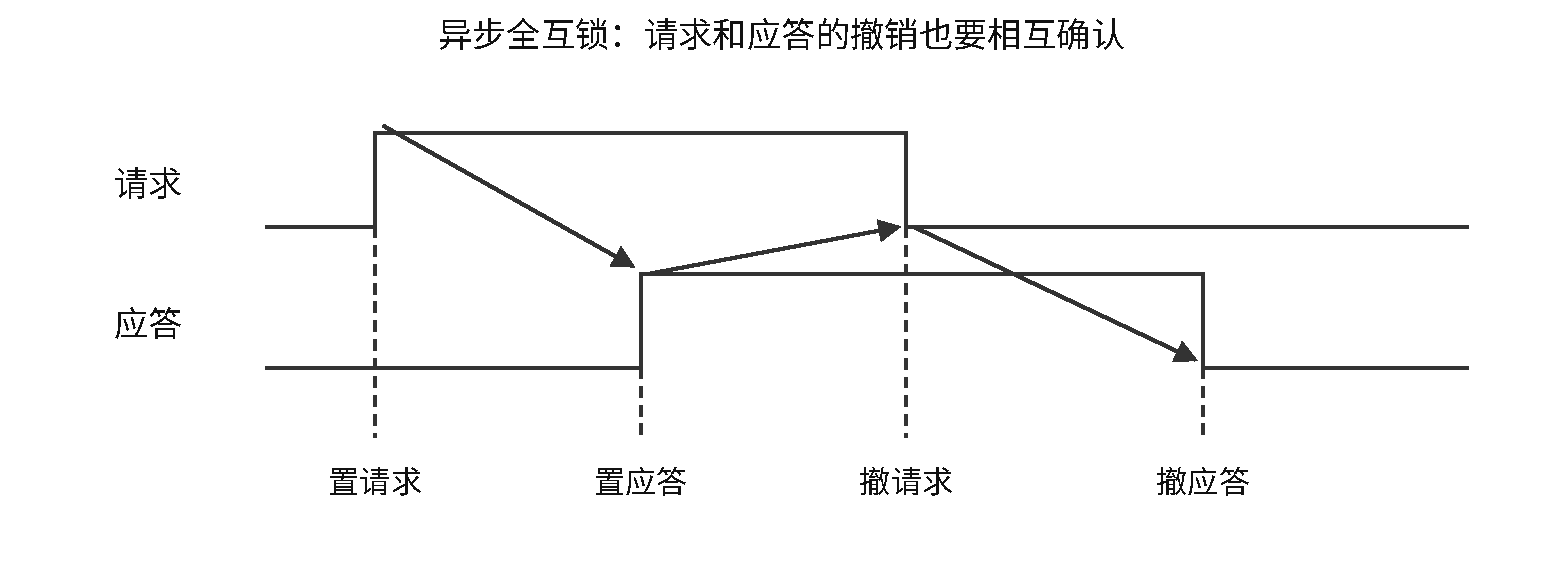
\includegraphics[width=\linewidth,height=125mm,keepaspectratio]{figures/CO_F10_bus_handshake.pdf}
\captionof{figure}{全互锁握手的撤销顺序也由对方信号确认}\label{co-fig-handshake}
\end{minipage}\par\medskip

非互锁方式中，主设备发出请求后按预定时间撤回，不等应答；从设备发出应答后也按时撤回，不等请求撤回。半互锁方式中，主设备等待应答出现才撤请求，而从设备仍可按时撤应答。全互锁方式中，从设备还必须等请求撤回才撤应答。给出时序图时，按图中信号的建立、撤销条件来识别，不单凭信号名称猜测。全互锁通常多了等待环节，不能因为最可靠就断定它最快。

半同步通信将时钟节拍与等待/应答结合：正常情况下按时钟节拍推进，慢设备可请求延长，握手状态在规定边沿采样。这里的``半同步''不等于一半数据串行、一半数据并行，两个分类维度不同。

\subsection{如何读总线时序图}\label{CO06-timeline}

先标出地址何时稳定、读写命令何时有效、数据何时有效和何时被接收，最后数出从事务开始到完成的时间。若图中低电平有效，应以标出的有效电平判断，不可把所有上升沿都当成开始。不同信号能否同拍出现由协议规定；``地址/数据复用''和``独立地址数据线''会改变哪些操作可以重叠。

串行异步字符传送每帧另加起始位和停止位，校验位可选。若每字符7个数据位、1个校验位、1个起始位和1个停止位，则每字符实际发送10位，480字符/s需要4800 bit/s，而有效字符数据只有3360 bit/s。不要把物理线路传送率与有效数据率混为一谈。

\subsection{事务速率巩固}\label{CO06-old-self}

\begin{enumerate}
\def\labelenumi{\arabic{enumi}.}
\tightlist
\item
  【配套例题】 某存储器总线采用同步通信，时钟频率50 MHz，突发传8个字，每字4 B。1周期接收地址、3周期等待、8周期传8个字。数据传输速率为（　）。A. 114.3 MB/s　B. 126 MB/s　C. 133.3 MB/s　D. 144.3 MB/s。
\item
  【配套例题】：将第1题改为每个字都独立付1周期地址、3周期等待、1周期数据，读同样8字需要多少时间，有效速率多少？
\end{enumerate}

\textbf{答案。} 1. C。共12周期，每周期20 ns，32 B/240 ns≈133.3 MB/s。2. 共40周期=800 ns，32 B/800 ns=40 MB/s。两题块长相同，改变的是启动代价的重复次数。

\section{总线仲裁与分离事务}\label{CO06-arbitration}

总线传输在申请分配阶段处理多个主设备的使用权竞争，随后寻址、传输并结束。CPU和DMA都可能成为主设备，主设备与从设备的角色针对一次事务；主设备申请总线，不表示它一定是本次数据的接收者。

课件将仲裁分为集中与分布两类。集中仲裁由一个仲裁部件授予使用权：链式查询以允许信号沿设备链传递，靠近仲裁端的请求通常先被满足，控制线少但固定优先级可能使低位请求长期等待；计数器定时查询依次给出设备号，请求者在号码匹配时取得资格，起始编号和轮转规则决定公平性；独立请求为各设备设置请求/允许通路，仲裁灵活但线路及逻辑开销较大。分布仲裁由参与者依共同规则竞争或判定，不能因此推断系统没有任何仲裁规则。

课件把总线仲裁与标准列为拓展。本章保留其机制联系，不凭文件名替读者确认某一考试年度的正式范围。总线标准还约定接口、电气、功能、时序等兼容条件；串行或并行只说明传输组织，不能单独决定峰值带宽或延迟。

分离事务允许主设备发出请求后释放总线，待从设备准备好再申请并返回结果；因此``总历时''与``总线实际占用时间''可以不同。它与普通同步/异步定时的分类角度不同，还需要标识请求与响应的对应关系。

\begin{wideblock}

\par\medskip\noindent\begin{minipage}{\linewidth}\fontsize{9.3}{12}\selectfont\begin{tabularx}{\linewidth}{@{}YYYY@{}}
\toprule\noalign{}
\begin{minipage}[b]{\linewidth}\raggedright
定时/组织
\end{minipage} & \begin{minipage}[b]{\linewidth}\raggedright
推进依据
\end{minipage} & \begin{minipage}[b]{\linewidth}\raggedright
等待是否占通路
\end{minipage} & \begin{minipage}[b]{\linewidth}\raggedright
不能直接推出
\end{minipage} \\
\midrule\noalign{}


同步 & 规定时钟沿；慢设备可插等待 & 由事务协议决定 & 每事务固定一拍 \\
异步全互锁 & 请求/应答建立和撤销均互相确认 & 由握手占用规则决定 & 不需要时序约束 \\
半同步 & 时钟节拍与等待/应答结合 & 需看等待状态的保持规则 & 一半串行一半并行 \\
分离事务 & 请求与响应分开争用通路 & 准备期间可释放 & 总历时等于占用时长 \\
\bottomrule\end{tabularx}
\end{minipage}\par\medskip

\end{wideblock}

\section{主动回忆自测}\label{CO06-recall}

{\tcbset{SNbase/.append style={breakable=false}}\begin{recallcard}[沿导图回答，再核对单位与条件]

以下为自拟检查，先遮住答案，按导图主枝回答。

\begin{enumerate}
\def\labelenumi{\arabic{enumi}.}
\tightlist
\item
  地址、数据、控制三类线的分工，是否按所传信息名称里有没有``控制''二字决定？
\item
  为什么32位、每拍两次的100 MHz总线，理想峰值是800 MB/s，而不是400 MB/s？
\item
  给200 MT/s后，能否因``每拍两次''再乘2？
\item
  连读8个字时，突发方式节省的是哪类重复开销？
\item
  全互锁握手四个事件的先后顺序是什么？
\item
  一次读请求等待100 ns，能否直接断言总线被独占100 ns？
\item
  仲裁与定时分别解决哪两个问题？
\item
  双向合计带宽与单方向带宽相差多少，是否总能用同一个倍数转换？
\end{enumerate}

\subsection{自测答案}\label{CO06-recall-answers}

\begin{enumerate}
\def\labelenumi{\arabic{enumi}.}
\tightlist
\item
  不能；命令字、状态字等编码值可走数据线，控制线规定事务类型和时序。2. 每次4 B，每秒 \(2\times100\times10^6\) 次，乘得800 MB/s，前提是全部数据位均有效。3. 不能，MT/s已经计入实际传送次数。4. 首地址、启动与准备等是否只付一次，由题设确定；数据拍仍要逐项数。5. 请求置位、应答置位、请求撤销、应答撤销。6. 不能，分离事务可在设备准备时释放总线。7. 谁获得使用权；何时采样与推进。8. 需看全/半双工、两个方向是否能同时达到峰值以及题目统计口径，不可无条件翻倍。
\end{enumerate}

\end{recallcard}}
